\section{Data mining}
Given data, find a model that matches the data.

\subsubsection{Challenges}
Transform masses of data into actionable intelligence.
\begin{itemize}
\item From TX data to market insights
\item From observations to scientific hypotheses
\item From usage data to better UI
\end{itemize}

Analysis of large data sets to find relationships and summarize data
in useful ways.

\begin{itemize}
\item Data access and domain knowledge
\item Data management (\textbf{Big Data})
\item Data mining : algorithms to extract rules and knowledge from data
\end{itemize}

\textbf{Examples}
\begin{itemize}
\item shopping basket analysis (60\% of people who buy diapers buy
  beer)
\item Analysis of query logs for query expansion.
\end{itemize}

\subsubsection{Classes of mining problems}
\begin{itemize}
 \item [\textbf{Local properties}]
\item Pattern that applies to part of the data
  \quad \item E.g.\ buy diapers $ \rightarrow $ buy beers
  Global model
\item Descriptive \textbf{structure} of the data
  \quad \item 3 types of customer behaviour
\item Predictive \textbf{function} of the data
  \quad \item dist(beer, diapers) = 1 $ \rightarrow $ + 10\% beer sales
\end{itemize}

\subsubsection{Components of mining algorithms}
\begin{itemize}
\item Pattern structure/model representation (\textbf{what} we look for?)
\item Scoring function (\textbf{how} well the model fits?)
\item Optimisation and search (\textbf{how} to tune the parameters of
  the model?
\item Data management (\textbf{how} to handle such large quantities of
  data)
\end{itemize}

\subsection{Association rule mining}
\subsubsection{Pattern structure}

We search for rules of the form: $ body \rightarrow Head[support,
confidence] $
\begin{itemize}
\item Body: predicate $ (x, x \in {items}) $
\item Head: predicate $ (x, x \in {items}) $
\item Support, confidence: measure of the rule's validity
  Example: $ buy(x, {diapers}) \rightarrow buy(x, {beer})[0.5\%, 60\%]
  $ \\
  Rules can be multi-dimensional e.g.\ $ body = age(x, {19-25}) \land
  buy(x, {chips}) \rightarrow buy(x, {coke})[10\%, 75\%] $
\end{itemize}

\subsubsection{Scoring function}

\textbf{Support}: probability that body and head occur in transaction
$ P(body \land head) $ \\
\textbf{Confidence}: probability that if body occurs, head also occurs
$ P(head \mid body) $

\subsubsection{Definition of association rules}
\begin{itemize}
\item [Terminology and notation]
\item set of all items I, subset of I called \textbf{itemset}
\item \textbf{Transaction}(tid, T), $ T \subseteq I $
\item Set of all transactions D (\textbf{database}), Transaction $ T
  \in D $
  \textbf{Association rules}: $ A \rightarrow B[s, c] $
\item A, B itemsets
\item $ A \cap B = \emptyset $
\item $ s = p(A \cup B) = \frac{count(A \cup B)}{\mid D \mid} $
\item $ c =  p(B \mid A) = \frac{count(A \cup B)}{count(A)} $
\end{itemize}

\textbf{Problem definition} \\
Given a database D of transaction (tid, T), find \\
\begin{itemize}
\item all rules $ A \rightarrow B[s, c] $
\item such that $ s > s_{min} $
\item and $ c > c_{min} $

\end{itemize}

\subsection{Mining approach}
\textbf{Two steps}
\begin{itemize}
\item Find \textbf{frequent} itemsets \\
  \quad $ J \subseteq I s.t.\ p(J) < s_{min} $
\item Select \textbf{pertinent} rules \\
  \quad $ A \rightarrow B s.t.\ A \cup B = J $ \\
  \quad and $ p(B \mid A) > c_{min} $
\item $ A \rightarrow B $ can be a rule only if $ A \cup B $ is
  frequent itemset
\item Any subset of a frequent itemset is a frequent itemset
  \textbf{Apriori property}
\item Find frequent itemsets with increasing cardinality from 1 to k
  to reduce search space.
\end{itemize}

\subsubsection{Exploiting the apriori property}
  Knowing (k-1)-itemsets, which are frequent k-itemsets?
\begin{itemize}
\item Any (ordered) (k-1)-itemsets that is a subset of X must be frequent
\item In particular two ordered (k-1)-itemsets that are subsets of X
  and differ only in last position must be frequent.
\item Thus, the union of two (k-1)-itemsets that differ only by one
  item is \textbf{candidate} frequent k-itemsets. \\
  Example: \{beer\} and \{milk\} differ by one, thus \{beer, milk\} is
  a candidate 2-itemset. \\
  \textbf{JOIN} set
\item Sort the itemsets in $ L_{k-1} $
\item Find all pairs with the same first k-2 items, but different
 $ k-1^{th} $ item
\item Join the two itemsets in all pairs and add to $ C_k $
  (\textbf{candidate set})
  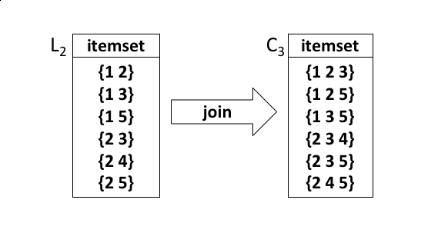
\includegraphics[height=150px,width=210px]{join}
  \\
  \quad \textbf{PRUNE} step
  A k-itemsets in $ C_k $ might still contain (k-1)-itemsets that are not
  frequent (k-1)-itemsets. \textbf{PRUNE} them. \\
  \quad \textbf{Final} step,
\item For the remaining k-itemset in $ C_k $ eliminate those that are not
  frequent by counting their occurences. \textbf{most expensive} but
  performed on small number of candiates, reduced by \textbf{JOIN} and
  \textbf{PRUNE}.
\end{itemize}

\subsubsection{Aprio algorithm}
\begin{lstlisting}[language=C,mathescape=true]
  k := 1, L_k := $ \{J \subseteq I : \mid J \mid = 1 \land p(J) > s_{min} \} $
  while $ L_k \neq \emptyset $ {
    $ C'_{k+1} $ := JOIN($ L_k $)
    $ C_{k+1} $ := PRUNE($ C'_{k+1} $)
    for all (id, T) $ \in $ D {
      for all $ J \in C_{k+1}, J \subseteq T $ {
        count(J)++
      }
    }
    $ L_{k+1} := \{ J \subseteq C_{k+1} : p(J) > s_{min} \} $
    k := k +1
  }
  return $ \bigcup_k L_k $
\end{lstlisting}

\subsection{Rule selection}
\begin{lstlisting}[language=C,mathescape=true]
  R := $ \emptyset $
  L := apriori(D)

  for($ J \in L $) {
    for($ A \subseteq J, A \neq \emptyset $) {
      r := $ A \rightarrow J \setminus A $
      if (c(r) = s(J) / s(A) > $ c_{min} $) {
        R := $ R \cup r $
      }
    }
  }
\end{lstlisting}

\subsubsection{Alternative measure of interest}
Added value (A,B itemsets)
$ AV(A \rightarrow B) = confidence(A \rightarrow B) - support(B) $ \\

Alternative: $ Lift(A \rightarrow B) = \frac{confidence(A \rightarrow
  B)}{support(B)} $

\subsection{Quantitative attributes}
Transforming quantitative values into categorical ones
\begin{itemize}
\item \texttt{Static discretization} predefined bins
\item \texttt{Dynamic discretization} based on distribution of the
  data
\end{itemize}

The rules depends on chosen discretization!!

\subsection{Improving apriori for large datasets}
\begin{itemize}
\item Transaction reduction: A TX that does not contain any frequent
  k-itemset is useless in subsequent scans
\item Sampling: mining on a sampled subset of DB, with lower support
\item Partitioning (SON algorithm): Any itemset that is potentially
  frequent in a DB must be frequent in at least one partition of the
  DB.
\end{itemize}

\subsubsection{Sampling}
Approach
\begin{itemize}
\item RAndomly sample transactions with proba p
\item Detect frequent itemset with support $ p \times s $
\item Eliminate \textbf{false positives} by counting frequent itemsets
  on complete data
\end{itemize}

Refinements
\begin{itemize}
\item If we assume the m TX are sorted randomly we can just choose the
  first $ p \times m $ ones
\item False negatives can be reduced by choosing a lower threshold,
  e.g.\ $ 0.9 \times p \times s $
\end{itemize}

\subsubsection{Partitioning}
\begin{itemize}
\item Divide transactions in $\frac{1}{p}$ partitions and read
  partitions in main memory
\item Use in-memory algorithm to find all frequent itemsets with
  support threshold $ p \times s $
\item An itemset becomes a candidate if it is found to be frequent in
  at least one partition
\item On a \textbf{second pass}, count all the candidate itemsets and
  determine which are frequent in the entire set.
\end{itemize}

\textbf{Why it works?}
\begin{itemize}
\item an itemset cannot be frequent in the entire set of TXs unless it
  is frequent in at least one partition
\item Proof: If $ \forall $ partitions support is below $ p \times s $
  the total support is less than $ \frac{1}{p} p \times s = s $ !
\item Partioning can be easily implemented using MapReduce!
\end{itemize}

\subsection{FP Growth}

Frequent itemset generation without candidate generation
\begin{itemize}
\item Build an FP-tree (2 passes over dataset)
\item Extract frequent itemsets from the FP-tree
\end{itemize}

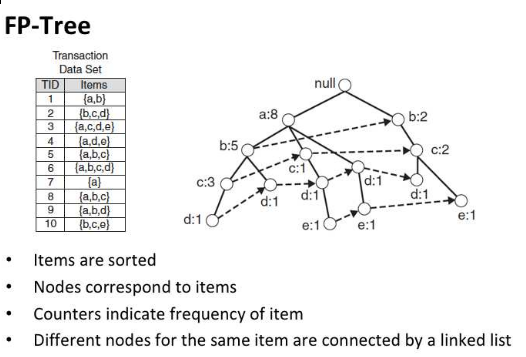
\includegraphics[height=120px, width=190px]{fptree}

\subsubsection{FP-Tree construction}

FP-tree size: the FP-tree is more compact the more common prefixes the
itemsets share. Sorting by \textbf{decreasing support} increases this
probability

\begin{itemize}
\item Pass 1:
  \quad \item Compute support for each item
  \quad \item Sort items in order of decreasing support
\item Pass 2:
  \quad \item Tree is expanded one itemset at a time
\end{itemize}

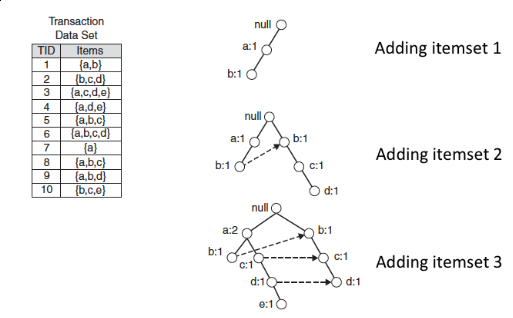
\includegraphics[height=150px, width=200px]{fpcon}
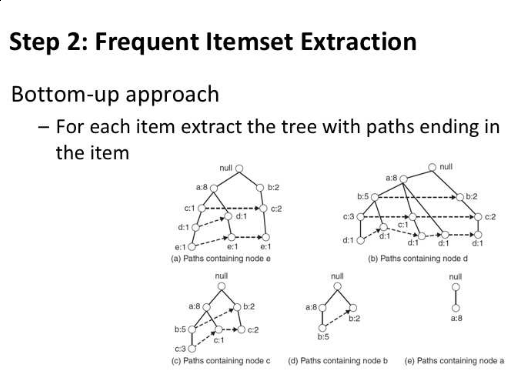
\includegraphics[height=150px, width=220px]{fpextract}

\subsection{Divide and conquer}
Start with item e with lowest support \\
Check whether it has sufficient support
\begin{itemize}
\item Add up counts along the list of the item
\item Then check if item has enough support
\item if not we know that no itemset containing 3 has sufficient
  support
\item if sufficient support, check for itemsets ending in the item
  \quad \item If item is frequent check for \textit{be},
  \textit{ce}\ldots
\end{itemize}

Derive \textbf{conditional FP-Trees}
\begin{itemize}
\item Update support counts to itemsets containing the item
\item Remove the node of the item
\item Remove nodes with insufficient support count
\end{itemize}

Another way to understand the construction of conditional FP-Tree is
that it is the FP-Tree that would be constructed when we only consider
the TX that consider the current item (or itemset) and then remove e
and any non-frequent item from those itemsets.

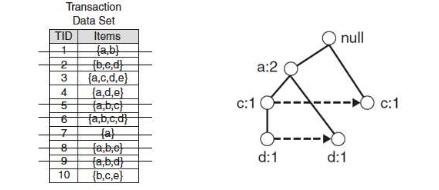
\includegraphics[width=200px, height=120px]{condfp}

In this example we consider item e, and item b would be eliminated
since not frequent in transactions.

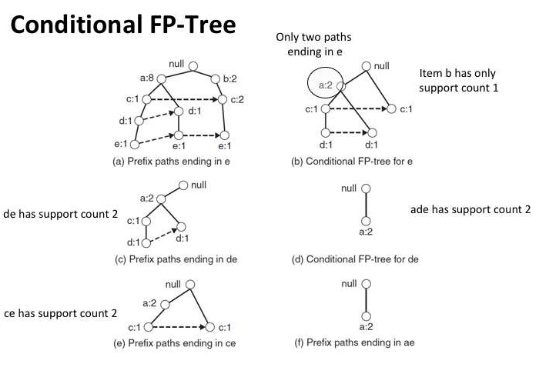
\includegraphics[width=220px, height=150px]{fpexample}

\subsection{Summary FP growth}
Advantages
\begin{itemize}
\item Only 2 passes
\item Compresses dataset
\item Generally much faster than apriori
\end{itemize}
Disadvantages
\begin{itemize}
\item Works less efficiency for high support thresholds
\item Has to run in main memory
\item Difficult to find distributed implementation
\end{itemize}


%%% Local Variables:
%%% mode: latex
%%% TeX-master: "master"
%%% End:
